\documentclass[%
 reprint,
%superscriptaddress,
%groupedaddress,
%unsortedaddress,
%runinaddress,
%frontmatterverbose, 
%preprint,
%showpacs,preprintnumbers,
%nofootinbib,
%nobibnotes,
%bibnotes,
 amsmath,amssymb,
 aps,
%pra,
%prb,
%rmp,
%prstab,
%prstper,
%floatfix,
]{revtex4-1}

\usepackage{graphicx}% Include figure files
\usepackage{dcolumn}% Align table columns on decimal point
\usepackage{bm}% bold math
%\usepackage{hyperref}% add hypertext capabilities
%\usepackage[mathlines]{lineno}% Enable numbering of text and display math
%\linenumbers\relax % Commence numbering lines

%\usepackage[showframe,%Uncomment any one of the following lines to test 
%%scale=0.7, marginratio={1:1, 2:3}, ignoreall,% default settings
%%text={7in,10in},centering,
%%margin=1.5in,
%%total={6.5in,8.75in}, top=1.2in, left=0.9in, includefoot,
%%height=10in,a5paper,hmargin={3cm,0.8in},
%]{geometry}

\usepackage{cmap} % Поиск в PDF
\usepackage[T2A]{fontenc} % Кодировка
\usepackage[utf8]{inputenc} % Кодировка исходного текста
\usepackage[english, russian]{babel} % Локализация и переносы
\frenchspacing % Более тонкая настройка пробелов 
\usepackage{multirow}
\usepackage[warn]{mathtext}
\usepackage{amssymb}
\usepackage{ dsfont }
\usepackage{ textcomp }
\usepackage{ mathrsfs }

% Переопределение англоязычного начертания каппа, фи и эпсилон, 
% а также знаков сравнения
\renewcommand{\epsilon}{\ensuremath{\varepsilon}}
\renewcommand{\phi}{\ensuremath{\varphi}} 
\renewcommand{\kappa}{\ensuremath{\varkappa}}
\renewcommand{\le}{\ensuremath{\leslant}}
\renewcommand{\leq}{\ensuremath{\leqslant}}
\renewcommand{\ge}{\ensuremath{\geslant}}
\renewcommand{\geq}{\ensuremath{\geqslant}}
\renewcommand{\emptyset}{\ensuremath{\varnothing}}

\usepackage{textcomp} 
\usepackage{indentfirst} % Красная строка
\usepackage{amsmath} % Текст в формулах
\usepackage{graphicx} % Графика
\DeclareGraphicsExtensions{.pdf,.png,.jpg}
\usepackage{pgfplots}
\pgfplotsset{compat=1.13}

%\usepackage{times}

\begin{document}

\title{Интерферометр Фабри-Перо}
\thanks{4.4.4}

\author{Иван Едигарьев}
\affiliation{
 Московский Физико-Технический Институт\\
 Факультет Общей и Прикладной Физики, 526т\\
}
%\date{\today}

\begin{abstract}
Цель работы: изучение интерферометра Фабри–Перо и определение его характеристик, как спектрального прибора.
В работе используются: интерферометры Фабри–Перо, линзы, светофильтр, ртутная лампа ПРК-2, высокочастотная натриевая лампа, катетометры КМ-6.

\end{abstract}

\pacs{Valid PACS appear here}

\maketitle

\begin{enumerate}

    \item 
    
    \textbf{Юстировка системы.}\\
    
    При измерении диаметров не рекомендуется определять координату центра системы колец, т.~к. погрешность этого определения велика. Измерения будут точнее, если, монотонно перемещая зрительную трубу снизу вверх, фиксировать координаты колец, начиная с самого дальнего от центра. Пройдя центр, последовательно фиксируем вторые координаты тех же колец. Удобно, пронумеровав предварительно кольца ($i = 1$ для центрального), записывать соответствующие одному кольцу координаты друг под другом.
    
    Так же измеряются диаметры колец от натриевой лампы. Средний диаметр близкой пары колец определяется последующим расчётом. 
    
    Измерим диаметры нескольких колец (6–8 пар колец для натриевой лампы).
    
    Для оценки разрешающей способности измерим ширину $\delta r(i)$ одного из колец, близких к центру.
    \begin{gather*}
        \delta r_{\downarrow} = 0.61 \, mm,\\
        \delta r_{\uparrow} = 0.62 \, mm.
    \end{gather*}
    
    Запишим фокусное расстояние линзы и величину L, указанные на установке.
    \begin{gather*}
        f = 94 \, mm,\\
        L = 0.1 \, mm.
    \end{gather*}
    
    \item 

    \textbf{Обработка результатов.}\\
    
    Построим график $d_i^2 = F(i)$. По наклону прямой определим $\lambda$ для интерферометра. \\
    \begin{figure}[h]
    \center{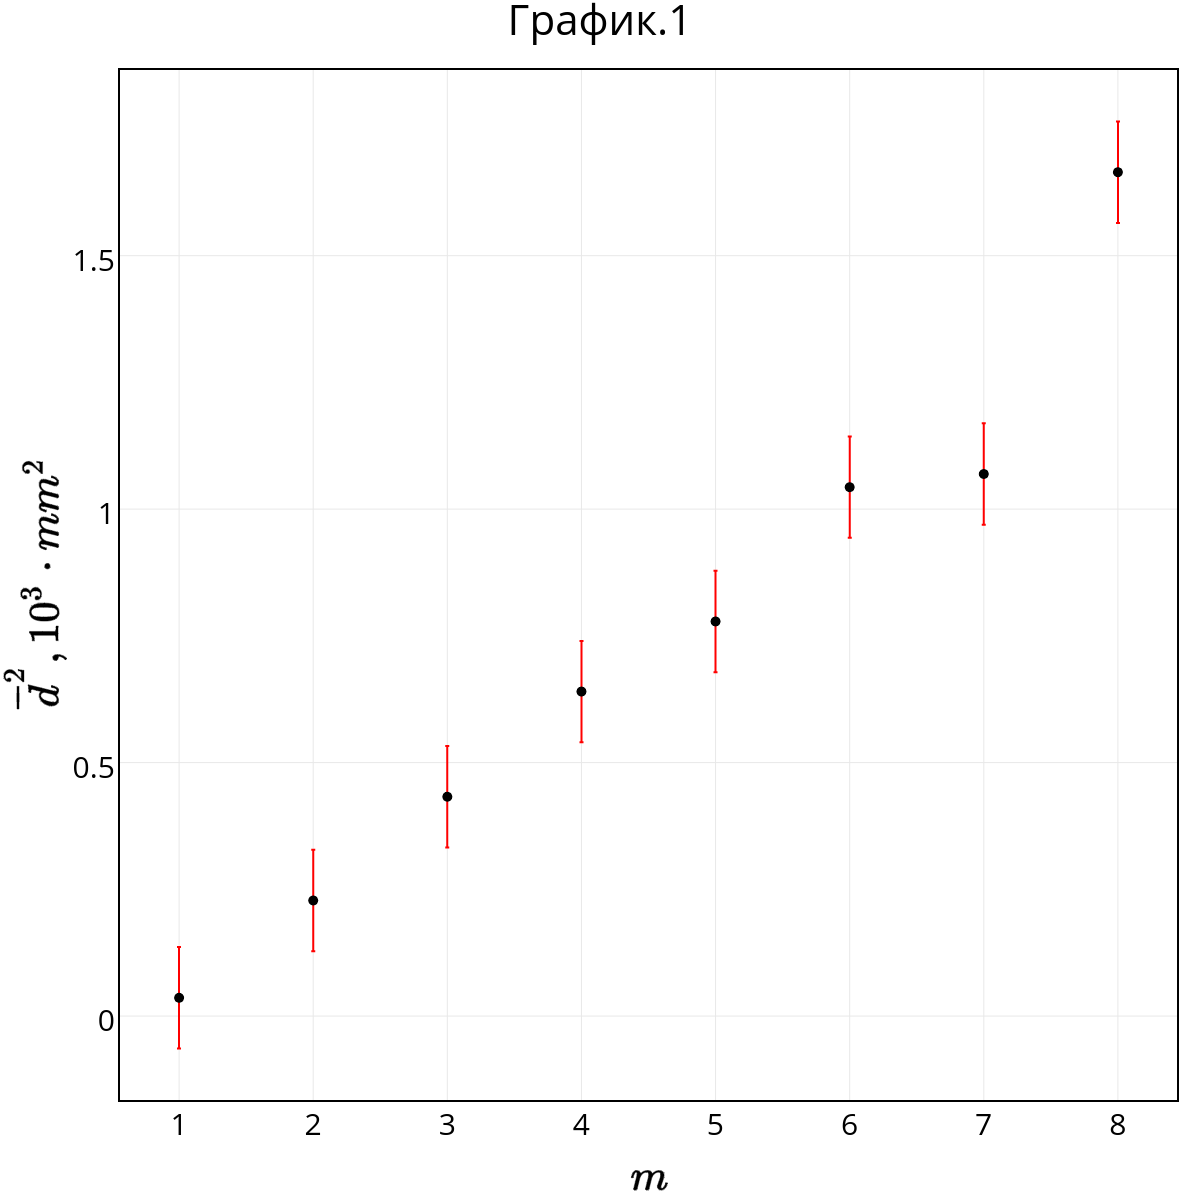
\includegraphics[scale=0.17]{my_plot1.png}}
    \end{figure}
    
    Воспользуемся методом наименьших квадратов, результат регрессии даётся одним коэффициентом наклона модельной прямой $b = \Delta(d_i^2) / \Delta(i)$ и свободным коэффициентом $a$:
    \begin{gather*}
        b = (209 \pm 2) \, mm.
    \end{gather*}
    Используя формулу
    \begin{gather*}
        \frac{\lambda}{L} = \frac{1}{4 f^2}\frac{\Delta(d_i^2)}{\Delta(i)}, 
    \end{gather*}
    получим оценку для $\lambda$:
    \begin{gather*}
        \lambda = (59 \pm 1) \cdot 10^2 \, \text{\AA}.
    \end{gather*}
    Сверим со значением приведённым на установке:
    \begin{gather*}
        \lambda = 5893 \, \text{\AA}.
    \end{gather*}
    Рассчитаем средние диаметры $\overline{d}$ и разности диаметров $\Delta d$ для колец одного порядка. Построим график $\overline{d} = F(1 / \Delta d)$. По углу наклона прямой рассчитаем разность длин волн $\Delta \lambda$.
    \begin{figure}[h]
    \center{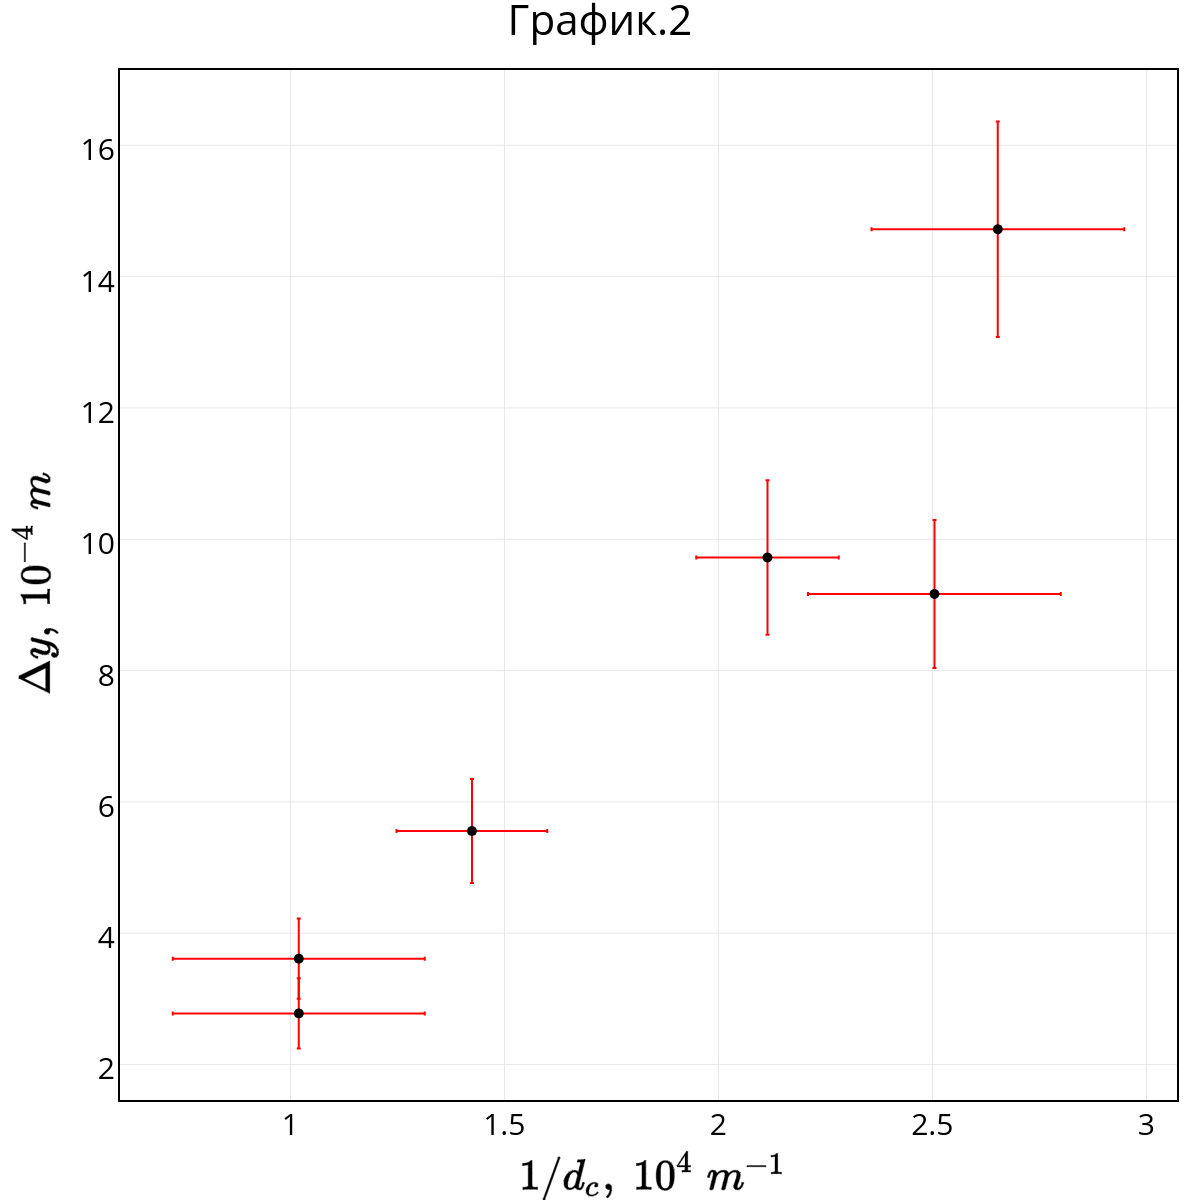
\includegraphics[scale=0.17]{my_plot2.png}}
    \end{figure}
    Проделаем аналогичную регрессию 
    \begin{gather*}
        b = (15 \pm 1)~mm^2.
    \end{gather*}
    Тогда
    \begin{gather*}
        \Delta \lambda_p = \frac{\lambda \overline{d} \Delta d}{4 f^2} = (2.5 \pm 0.4)~\text{\AA}.
    \end{gather*}
    Далее оценим экспериментальное значение линейной дисперсии интерферометра, используя разность диаметров и разность длин волн жёлтых пар.
    \begin{gather*}
        D^*_{\text{эксп}} = f\frac{d\theta}{d\lambda} = \frac{\Delta d}{2 \cdot \Delta \lambda} = (0.34 \pm 0.02)~\frac{mm}{\text{\AA}},\\
        D^*_{\text{теор}} = \frac{2 f^2}{\lambda d} = (0.12 \pm 0.1)~\frac{mm}{\text{\AA}}.
    \end{gather*}
    
    Оценим также аппаратную разрешающую способность, рассчитав $\delta \lambda$ через диаметр кольца $d$ и его ширину $\delta r$. Можно получить
    \begin{gather*}
        R_{\text{апп}} = \frac{\lambda}{\delta \lambda} \approx \frac{4 f^2}{d \cdot \delta r} = 9.9.
    \end{gather*}
    
    Также оценим число интерферирующих лучей по аналогии с решёткой:
    \begin{gather*}
        N = R_{\text{апп}} / m = 2.5.
    \end{gather*}
    
    Рассчитаем теоретическое значение добротности интерферометров, приням коэффициент отражения $r \approx 0.85$. Оценим также число интерферирующих лучей.
    \begin{gather*}
        R = \frac{\pi \sqrt{r}}{1 - r} m = 77, \\
        N = R / m = 19.
    \end{gather*}
    
    
    
\end{enumerate}

\end{document}
